%version of 07-08-19

\chapter{Graphs I:
Representing Relationships Mathematically}
\label{ch:Graphs1}
\index{graph}

Graphs provide one of the richest technical and conceptual frameworks
in the world of computing.  They provide concrete representations of
manifold data structures that should be studied in depth
\ignore{**hence must be well understood**}
in preparation for a ``Data Structures and Algorithms'' course.  They
embody tangible abstractions of relationships of all sorts, hence must
be well understood in order to discuss entities as varied as
web-search engines and social networks with precision and rigor.  As
with most of the topics we discuss in this text, graph-oriented
concepts must be taught ``in layers''.  All students should be
conversant with the use of graphs to represent and reason about a vast
array of complicated relationships---ranging from taxonomies
(including intra-family structures) to link-based data structures to
interconnectivity within social media, and on and on---but the degree
of sophistication that an individual student requires depends both on
the abilities of the student and the range of graph-modeled concepts
that will appear in the student's program.  The most-basic concepts in
this chapter should be understood by all students in any academic
program that includes a computation-oriented component---although each
concept can be developed with more texture and nuance within the
context of specific application domains; the more advanced concepts
should be selected with care, based on the instructor's perception of
students' needs, in the light of the ever-growing importance of
concepts involving interconnectivity.

Many developments in computing technology over recent decades have
made it imperative that graphs no longer be viewed by students as the
static objects introduced early in the history of computational
studies.  For instance, while it was innovative in the 1960s to employ
graphs and trees computationally as abstractions of data structures, such a view
is standard today.  Similar remarks, perhaps with differing dates, can
be made about graphs as vehicles for representing the flow of control
and information and as vehicles for representing interconnectivity
among both concepts and populations.  Applications ranging from
databases to web-search engines to social networks demand an
appreciation of graphs as dynamic objects.  This change in perspective
affects many aspects of the mathematical prerequisites for any
academic program that includes a computation-oriented component.

\section{Generic Graphs: Directed and Undirected}
\label{sec:graphs-generic}
\label{sec:basic-graphs}

\subsection{Connectivity-related concepts}
\label{sec:connectivity-notions}

% general introduction
The basic components of a graph $\g$ are \index{graph!nodes}
\index{graph!vertices} \index{node (of a graph)} \index{vertex (of a graph)} 
  its {\em nodes/vertices} (one encounters both terms in the
literature) and its {\em edges} \index{graph!edges}
\index{edge (of a graph)} that interconnect them.  (The singular form
of ``vertices'' is {\it vertex}.)  \index{graph!vertex} \index{vertex (of a graph)}

% undirected case
When graph $\g$ is {\em undirected}, \index{graph!undirected} each of
its edges connotes some sort of sibling-like relationship among nodes
of ``equal'' status.  When graph $\g$ is {\em directed}
\index{graph!directed} (sometimes referred to as a {\em digraph}),
\index{digraph} \index{graph!digraphs} each of its edges connotes an
``unequal'' relationship such as parenthood or priority or dependence;
edges in directed graphs are often termed {\em
  arcs}. \index{graph!arc} \index{arc (of a directed graph)}

In many situations involving directed graphs, it is important to
deal with the {\em reverse} \index{graph!digraph!dual} of a digraph $\g$. 
This new graph---which is usually denoted by some notational
embellishment of ``$\g$'', such as $\widehat{\g}$---is the digraph
obtained by {\em reversing} all of $\g$'s arcs.  One sometimes
encounters situations when arguments about, or operations on, a
digraph $\g$ can be ``translated'' to arguments about, or operations
on, $\widehat{\g}$ with only clerical effort.  A {\em subgraph} $\g'$
of a graph $\g$ is a graph whose nodes are a subset of $\g$'s and
whose edges are a subset of $\g$'s that interconnect only nodes of $\g'$.  
\medskip

{\em Undirected} graphs are usually the default concept, in the
following sense: When $\g$ is described as a ``graph,'' with no
qualifier ``directed'' or ``undirected,'' it is usually understood
that $\g$ is an undirected graph.
\medskip

A {\em path} \index{graph!path} \index{path (in a graph)} in
an undirected graph is a sequence of nodes within which every adjacent
pair is connected by an edge.  A path is a {\em cycle}
\index{graph!cycle} \index{cycle (in a graph)} if all nodes in the
sequence are distinct, except for the first and last, which are
identical.  Paths and cycles in directed graphs are defined similarly,
except that every adjacent pair of nodes must be connected by an arc,
and all arcs must ``point in the same direction.''
\bigskip

A {\it directed graph} \index{graph!directed} ({\it digraph},
\index{digraph} for short) $\g$ is given by a set of {\it nodes}
\index{graph!node}
\index{$\n_{\fg}$: set of nodes of graph $\g$}
$\n_{\fg}$ and a set of {\it arcs}
\index{graph!digraph!arcs}
(or {\it directed edges}) $\a_{\fg}$.
In the following, we will omit the subscript if there is no ambiguity.
\index{$\a_{\fg}$: set of arcs of digraph $\g$}
Each arc of $\g$ has the form $(u \rightarrow v)$,
\index{$\rightarrow$: arc in a directed graph}
where $u, v \in \n$; we say that this arc goes {\em from} $u$
{\em to} $v$.  A {\it path} 
\index{graph!path in a digraph}
\index{path in a digraph}
in the digraph $\g$ is a sequence of arcs that share adjacent
endpoints, as in the following $(n-1)$-arc path from node $u_1$ to
node $u_n$ in $\g$:
\begin{equation}
\label{eq:di-path}
(u_1 \rightarrow u_2), \ (u_2 \rightarrow u_3), \ \ldots, \ (u_{n-2}
        \rightarrow u_{n-1}), \ (u_{n-1} \rightarrow u_n)
\end{equation}
The path (\ref{eq:di-path}) is often written in the more succinct form
\[
u_1 \ \rightarrow \ u_2 \ \rightarrow \ u_3 \ \rightarrow \cdots
\rightarrow \ u_{n-2} \ \rightarrow \ u_{n-1} \ \rightarrow \ u_n
\]
The just-described path makes sense only when every node $u_i$ belongs
to $\n$ and every one of its arcs, $(u_i \rightarrow u_{i+1})$,
belongs to $\a$.  The {\it length} of path (\ref{eq:di-path}) is
the number of arcs, i.e., $n-1$.  The existence of the path means that
the {\it distance} \index{distance!in a digraph}
\index{digraph!distance} \index{graph!distance!in a digraph} from
$u_1$ to $u_n$ in $\g$ is no greater than $n-1$ (where the distance here is taken in term of number of arcs.  
Notice also there may exist shorter paths in $\g$ from $u_1$ to $u_n$.)
\bigskip

\noindent \fbox{
\begin{minipage}{0.95\textwidth}
In the presentation above, we implicitly considered that there are no
redundant vertices in a path.
This is obviously always possible since if a vertex appears twice, we simply skip the sub-path between these two occurrences.

{\Denis Do we introduce here few words here about the Koenig Lemma?}
\end{minipage}
}
\bigskip

It is sometimes useful to endow the arcs of a digraph with labels from
an alphabet $\Sigma$.  When so endowed, the path (\ref{eq:di-path})
would be written in a form such as

\smallskip

\hspace*{.35in}$\displaystyle
(u_1 \stackrel{\lambda_1}{\rightarrow} u_2), \ 
(u_2 \stackrel{\lambda_2}{\rightarrow} u_3), \ \ldots, \ 
(u_{n-2} \stackrel{\lambda_{n-2}}{\rightarrow} u_{n-1}), \ 
(u_{n-1} \stackrel{\lambda_{n-1}}{\rightarrow} u_n)$

\smallskip

\noindent
where the $\lambda_i$ denote symbols from $\Sigma$.  Labeled paths
also are often written in a succinct manner, as:

\smallskip

\hspace*{.35in}$\displaystyle 
u_1 \ \stackrel{\lambda_1}{\rightarrow} \ u_2
    \ \stackrel{\lambda_2}{\rightarrow} \ u_3
    \ \stackrel{\lambda_3}{\rightarrow} \ \cdots \ 
    \ \stackrel{\lambda_{n-3}}{\rightarrow} \ u_{n-2}
    \ \stackrel{\lambda_{n-2}}{\rightarrow} \ u_{n-1}
    \  \stackrel{\lambda_{n-1}}{\rightarrow} \ u_n$

\medskip

If $u_1 = u_n$, then we call path (\ref{eq:di-path}) a {\em (directed)
  cycle},\index{cycle (in a digraph)} and we call its labeled version
a {\em labeled (directed) cycle}.  (The qualifier ``directed'' is
usually included only for emphasis.)
\medskip

An {\em undirected graph} $\g$ is given by a set of nodes $\n$
and a set $\e$ 
\index{$\e_{\fg}$: the set of edges of the undirected  graph $\g$}
of $2$-element subsets of $\n$.  Each of these subsets is called
an {\it edge}.
\index{graph!edge} \index{edge (of a graph)}
One can, thus, view the undirected graph $\g$ as being obtained from a
directed graph $\bar{\g}$ by removing the directionality of
$\bar{\g}$'s arcs.  Whereas we say: \\
\hspace*{.35in}the {\em arc} $(u,v)$ goes {\em from} node $u$ {\em to}
node $v$ \\
we say: \\
\hspace*{.35in}the undirected edge $\{u,v\}$ goes {\em between} nodes
$u$ and $v$ \\
or, more simply: \\
\hspace*{.35in}the undirected edge $\{u,v\}$ {\em connects} nodes $u$
and $v$.  
\medskip

One can view an undirected graph as asserting ``pure'' connectivity,
whereas directed graphs assert some form of priority or directionality.

A {\it path} in an undirected graph 
\index{graph!path in undirected graph} \index{path in an undirected graph}
is a sequence of edges---i.e., of $2$-element sets of nodes---such
that adjacent edges share a node.  For illustration, an $(n-1)$-edge
path that connects nodes $u_1$ and $u_n$ in the undirected graph $\g$
has the form
\begin{equation}
\label{eq:undi-path}
\{u_1, u_2\}, \ \{u_2, u_3\}, \ \ldots, \ \{u_{n-2}, u_{n-1}\}, \ \{u_{n-1}, u_{n}\}
\end{equation}
The path described in (\ref{eq:undi-path}) makes sense only when every
node $u_i$ belongs to $\n$ and every edge $\{u_i \ u_j\}$ belongs
to $\e$.  The {\it length} of path (\ref{eq:undi-path}) is the
number of edges---which is $n-1$ here; and the existence of
the path means that the {\it distance} \index{graph!distance} 
\index{distance!in an undirected graph}
{\it between} $u_1$ and $u_n$ in $\g$ is no greater than $n-1$.  (There
may exist shorter paths that connect $u$ and $v$.)
\medskip

For each edge $\{u,v\} \in \e$, we call nodes $u$ and $v$ {\it neighbors} (in $\g$).
\index{graph!nodes!neighbor nodes}
\index{neighbor node!in a graph}
The {\it degree}
\index{graph!nodes!degree of a node in an undirected graph}
\index{graph!degree of a node in an undirected graph}
\index{degree of a node in an undirected graph}
of a node $u \in \n$ is the number of neighbors that $u$ has.

Even at this early moment in our study of graphs, we can observe a few
important facts that can be useful when analyzing a broad range of
computation-related issues involving graphs (either as auxiliary
notions or as subjects of discourse).

\begin{prop}
\label{thm:number-edges/arcs}
{\bf (a)}
An $n$-node digraph $\g$ has no more than $n^2$ arcs.

{\bf (b)}
An $n$-node graph $\g$ has no more than $\displaystyle {n \choose 2}$ edges.
\end{prop}

\begin{proof}
{\bf (a)}
The set $\a$ of arcs of $\g$ is a subset of the set of ordered
pairs of nodes of $\g$.  This latter number is clearly $n^2$, because
one can choose the first node in a pair in $n$ ways and then {\em
  independently} choose the second node in $n$ ways.
\medskip

\noindent {\bf (b)}
The stated number is the number of $2$-node subsets of $\n$.  To
wit, start by listing the $n^2$ ordered pairs of nodes of $\g$.
First, eliminate from the list all $n$ pairs whose first and second
elements are equal: a set of the form $\{ u,u\}$ has only one element,
hence is not an edge of $\g$.  Then, for each distinct pair of nodes
$u, v \in \n$, eliminate one of the two ordered pairs, $\langle
u,v \rangle$ and $\langle u,v \rangle$: both of these ordered pairs
lead to the same unordered set $\{ u,v\}$, hence the same edge of
$\g$.  After these eliminations, we are left with
\[ \frac{n^2 - n}{2} \ = \ {n \choose 2} \]
$2$-element subsets of $\n$, from which we choose the edges of
$\g$. \qed
\end{proof}


\begin{prop}
\label{thm:even-num-odd-degrees}
In any undirected graph, the number of nodes of odd degree is even.
\end{prop}

\begin{proof}
The result follows directly from the following equation that holds for
any undirected graph $\g$:

\[ \sum_{v \in {\cal N}_{\cal G}} \ \mbox{\sc degree}(v) \ = \ 2 \cdot
|\e_{\cal G}|.
\]
The equation holds because each edge $e$ of $\g$ ``touches'' two nodes
of $\g$, namely, $\e$'s two endpoints.  Since the sum of $\g$'s
node-degrees is even, each odd node-degree must be paired (in the sum)
with another odd node-degree.  \qed
\end{proof}

\medskip

We sometimes use the term {\it neighbor} within the context of {\em
  directed} graphs also.  If we say that nodes $u$ and $v$ are
neighbors in the directed graph $\g$,
\index{neighbor node!in a directed graph}
then we mean that $\a_{\fg}$ contains at least one of the arcs $(u
  \rightarrow v)$ or $(v \rightarrow u)$.  More typically, we use
  terminology that is more faithful to digraph $\g$'s directedness.
If $\a_{\fg}$ contains the arc $(u \rightarrow v)$, then we would call
  $v$ a {\it (direct) successor} of $u$
\index{digraph!successor node}
\index{successor node in a directed graph}
and we would call $u$ a {\it (direct) predecessor} of $v$
\index{digraph!predecessor node}
\index{predecessor node in a directed graph}
The term {\it parent} often replaces ``predecessor node'', and the
term {\it child} often replaces ``successor node'', especially when
$\g$ is a directed {\em tree}.  Acknowledging the distinction between
predecessors and successors in digraphs, we usually split the notion
of the degree of a node within a digraph into the {\it indegree} and
the {\it outdegree} of node $u$:
\begin{itemize}
\item
The {\it indegree} of node $u \in \n_{\fg}$
\index{digraph!indegree}
is the number of nodes $v \in \n_{\fg}$ such that $(u \rightarrow v)$
is an arc of $\g$.
\item
Symmetrically, the {\it outdegree} of node $u \in \n_{\fg}$
\index{digraph!outdegree}
is the number of nodes $v \in \n_{\fg}$ such that $(v \rightarrow u)$
is an arc of $\g$.
\end{itemize}

\smallskip

The reader will note that we nowhere guarantee that there is always a
path that connects each node $u$ with each other node $v$.  We say
that a graph $\g$ is {\it connected} \index{graph!connected} if every
pair of nodes $u, v \in \n_{\fg}$ is connected by a path in $\g$.  If
graph $\g$ is {\em not} connected, then it is the disjoint union of
some number $c$ of connected subgraphs, usually called $\g$'s {\it
  (connected) components}.  \index{graph!connected components} Of
course, $\g$ is connected just when $c=1$; i.e., there is a single
connected component.


%%%%%%%%%%%%%%%%%%%%%%%%%%%%%%%%%%%

\subsection{Graphs as a modeling tool: the {\sf 2SAT} problem}
\label{sec:graph-model-2SAT}

Now that we have the basic notions relating to connectivity in graphs,
we can develop the proof of Proposition~\ref{thm:2SAT}.  For the
reader's convenience, we restate the Proposition here.

\begin{prop}{Restatement of Proposition~\ref{thm:2SAT}}
\label{thm:2SAT-reprise}
The {\sf 2SAT} problem can be solved in polynomial time.

\noindent
That is, given any instance $\Phi$ of {\sf 2SAT}, one can determine in
time polynomial in the number of literals in $\Phi$ whether there
exists a satisfying assignment of truth-values to the variables of
$\Phi$.
\end{prop}

We develop the proof of Proposition~\ref{thm:2SAT-reprise} by focusing
on an instance of the {\sf 2SAT} problem: the following POS expression
for a propositional formula $\Phi$:
\begin{eqnarray}
\label{eq:Phi-2SAT}
\Phi & = & C_1 \ \wedge \ C_2 \ \wedge \cdots \wedge \ C_m \\
\nonumber
  & \mbox{where:} & \bullet \ \ \mbox{each clause }
 \ C_i \ = \ \ell_{i,1} \vee \ell_{i,2} \\
\nonumber
  &               & \bullet \ \ \Phi \ \ \mbox{ has $n$ logical variables}
\end{eqnarray}
We transform $\Phi$ into a directed graph $\g(\Phi)$ that has $2n$
vertices and $2n$ arcs.
\begin{itemize}
\item
For each logical variable, $x$: there is one vertex that represents
the {\sc true} literal form, $x$, of variable $x$, and a second vertex
that represents the {\sc false} literal form, $\bar{x}$, of the
variable.
\item
Each clause $C_i = (\ell_{i,1} \vee \ell_{i,2})$ is represented by a
pair of arcs.  Say that literal $\ell_{i,1}$ comes from variable
$x_1$, and literal $\ell_{i,2}$ comes from variable $x_2$.  These arcs
represent ``instructions'' for assigning truth-values in a way that
maximize the number of clauses that receive the value {\sc true}.
  \begin{itemize}
  \item
There is an arc $(\bar{x_1} \rightarrow x_2)$.

This arc indicates that, if variable $x_1$ is assigned truth-value
{\sc false}, then variable $x_2$ should be assigned truth-value {\sc
  true}.
  \item
Symmetrically, there is an arc $(\bar{x_2} \rightarrow x_1)$.

This arc indicates that, if variable $x_2$ is assigned truth-value
{\sc false}, then variable $x_1$ should be assigned truth-value {\sc
  true}.
  \end{itemize}
\end{itemize}
All paths in $\g(\Phi)$ represent logical implications. 

The core of our proof is the following result.

\begin{prop}
\label{prop:2SAT}
The POS formula $\Phi \ = \ C_1 \ \wedge \ C_2 \ \wedge \cdots \wedge
\ C_m$ is satisfiable if, and only if, no strongly connected component
of $\g(\Phi)$ contains both the positive form ($x$) and the negated
form ($\bar{x}$) of any variable $x$ of $\Phi$.
\end{prop}

The proof is a consequence of the two following elementary results.

\begin{lemma}
\label{lem:2SATlemma1}
If $\g(\Phi)$ contains a path from vertex $x$ to vertex $y$, then it
contains a path from vertex $\bar{y}$ to vertex $\bar{x}$.
\end{lemma}

The proof, by induction on the length of the shortest path from vertex
$x$ to vertex $y$, is left to the reader. 

\begin{lemma}
\label{lem:2SATlemma2}
If $\g(\Phi)$ contains a path from vertex $x$ to vertex $y$, then for
every truth assignment $t$ that satisfies formula $\Phi$ (i.e.,
evaluates $\Phi$ to {\sc true}), if $t$ assigns variable $x$ the
truth-value {\sc true}, then $t$ also assigns variable $y$ the
truth-value {\sc true}.
\end{lemma}

\begin{proof}
Assume that $\Phi$ is satisfied by a truth assignment $t$ which
assigns variable $x$ the truth-value {\sc true}.  Say, for
contradiction, that along the path from $x$ to $\bar{x}$ in
$\g(\Phi)$, there exists an arc (say $(\alpha \rightarrow\beta)$) such
that assignment $t$ assigns the value {\sc true} to $\alpha$ and the
value {\sc false} to $\beta$.  Because of the way we constructed
$\g(\Phi)$, the existence of this arc means that $\Phi$ contains the
clause $\bar{\alpha} \vee \beta$.  Moreover, under truth assignment
$t$, this clause of $\Phi$ evaluates to {\sc false}, because both of
its literals are assigned value {\sc false}.  This contradicts the
assumption that $t$ is a satisfying assignment for $\Phi$.  \qed
\end{proof}

We finally prove the main result of this section,
Proposition~\ref{prop:2SAT}.

\begin{proof}[Proposition~\ref{prop:2SAT}]
Focus on a POS formula $\Phi$ and its associated digraph $\g(\Phi)$.

{\bf Necessity}.
Say first that $\g(\Phi)$ has a strongly connected component which
contains vertices arising from a variable $x$ in both positive ($x$)
and negated ($\bar{x}$) forms.  We claim that $\Phi$ is not
satisfiable.

Now, by definition of ``strongly connected'', $\g(\Phi)$ must contain
paths between the vertices corresponding to $x$ and $\bar{x}$.  By
Lemma~\ref{lem:2SATlemma2}, therefore, any truth-assignment that could
satisfy formula $\Phi$ would have to assign literals $x$ and $\bar{x}$
the same truth-value.  Any such truth-assignment to formula $\Phi$'s
{\em literals} would not be a valid truth-assignment to $\Phi$'s {\em
  variables} (specifically to variable $x$).  We conclude that no
valid truth-assignment could satisfy formula $\Phi$.

\medskip

{\bf Sufficiency}.
Say next that $\g(\Phi)$ has no strongly connected component which
contains vertices arising from a variable $x$ in both positive ($x$)
and negated ($\bar{x}$) forms.  We construct a truth-assignment $t$ to
$\Phi$'s variables under which $\Phi$ evaluates to {\sc true}.
Assignment $t$ witnesses $\Phi$'s satisfiability.

We construct a satisfying truth-assignment $t$ for $\Phi$ as follows.

\noindent {\bf 1.}
Say that graph $\g(\Phi)$ has $k$ mutually disjoint strongly connected
components.  We label these components in {\it topological order},
\index{topological order} as $S_1, S_2, \ldots, S_k$.  The phrase
{\it ``topological order''} means the following.
\begin{itemize}
\item
$\g(\Phi)$ contains no arc of the form $(u \rightarrow v)$ where
  vertex $u$ belongs to some component $S_i$, and vertex $v$ belongs
  to some component $S_j$ with $j < i$.
\end{itemize}
We know that this labeling is possible because any such arc would make
all vertices of $S_j$ accessible from all vertices of $S_i$, and
conversely.  This would mean that $S_i$ and $S_j$ would be contained
within the same strongly connected component---which would contradict
their assumed disjointness.
\medskip

\noindent {\bf 2.}
We assign truth-values to variables of $\Phi$ by scanning the
vertices/literals of $\g(\Phi)$ in decreasing order of the topological
indices of $\g(\Phi)$'s strongly connected components.
\begin{itemize}
\item
The {\em first time} that we encounter a vertex/literal $\ell$, in
true or negated form, we assign the truth-value to $\ell$'s associated
variable that makes literal $\ell$ {\sc true}.  This strategy also
makes the clause that this instance of literal $\ell$ occurs in
evaluate to {\sc true}.
\item
If we encounter an instance of a vertex/literal $\ell$ whose
associated variable has already been assigned a truth-value, then we
assign to this instance a truth-value that is consistent with the
variable's assignment: a positive literal gets the same assignment,
while a negative instance gets the negated version of the assignment.
\end{itemize}

Proceeding in this fashion, we develop a truth-assignment that
satisfies all of $\Phi$'s clauses.  To wit, assume for contradiction
that some clause of $\Phi$, say $(\xi \vee \eta)$, is not satisfied
under our procedure.  This means, in particular, that our assignment
$t$ assigns the truth-value {\sc false} to vertex/literal $\xi$.  But,
this can happen only if $t$ has assigned the truth-value {\sc true} to
vertex/literal $\bar{\xi}$, within a strongly connected component of
$\g(\Phi)$ whose index is higher than that of the strongly connected
component that $\xi$ occurs in.  The same observation applies to
vertex/literal $\eta$.  But this is impossible, because within our
construction of $\g(\Phi)$, the clause $(\xi \vee \eta)$ in formula
$\Phi$ would add the arc $(\bar{\xi} \rightarrow \eta)$ to graph
$\g(\Phi)$.  It follows that we have found a truth assignment that
satisfies formula $\Phi$, as was claimed.  \qed
\end{proof}

\medskip

We close with two small examples to illustrate
Proposition~\ref{prop:2SAT}
\begin{enumerate}
\item
Fig.~\ref{2SATyes} illustrates $\g(\Phi_1)$, for the formula
\[ \Phi_1 \ = \ (\bar{x}_{3} \vee \bar{x}_{1}) \ \wedge \
 (x_{1} \vee \bar{x}_{2}) \ \wedge \ (x_{2} \vee x_{3})
\]
The graph has the two strongly connected components illustrated in the
figure.  One can thereby read off the following satisfying truth-value
assignment $t$ for formula $\Phi_1$: $t(x_1) = \mbox{\sc false}$;
$t(x_2) = \mbox{\sc false}$; $t(x_3) = \mbox{\sc true}$.
\begin{figure}[htb]
\begin{center}
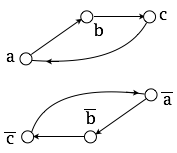
\includegraphics[width=0.3\textwidth]{FiguresGraph/2SATyes.png}
\caption{A portion of the digraph $\g(\Phi_1)$.  The graph's two
  strong components provide a truth assignment for $\Phi_1$: $t(x_1) =
  \mbox{\sc false}$; $t(x_2) = \mbox{\sc false}$; $t(x_3) = \mbox{\sc
    true}$.}
\label{2SATyes}
\end{center}
\end{figure}

\item
Fig.~\ref{2SATno} illustrates $\g(\Phi_2)$, for the formula
\[ \Phi_2 \ = \ (\bar{x}_{3} \vee \bar{x}_{1}) \ \wedge \                                      
(\bar{x}_{1} \vee x_{3}) \ \wedge \ (x_{2} \vee x_{3})
\]
Because the graph contains a (directed) path from vertex $x_1$ to
vertex $\bar{x}_1$, Proposition~\ref{prop:2SAT} assures us that formula
$\Phi_2$ does not admit any satisfying truth-assignment.
\begin{figure}[h]
\begin{center}
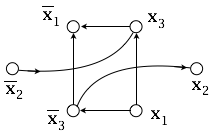
\includegraphics[width=0.3\textwidth]{FiguresGraph/2SATno.png}
\caption{A portion of the digraph $\g(\Phi_2)$.  Because the graph
  contains  a path from vertex $x_1$ to vertex $\bar{x}_1$,  formula
  $\Phi_2$ does not admit any satisfying truth-assignment.}
\label{2SATno}
\end{center}
\end{figure}
\end{enumerate}

\medskip

Even without formal background in algorithmics, it is clear that the
processes of: constructing digraph $\g(\Phi)$ from formula $\Phi$;
isolating and investigating the strongly connected components of
$\g(\Phi)$ can be accomplished in a number of computational steps that
is polynomial in the size of $\Phi$.  This validates
Proposition~\ref{prop:2SAT}.  \qed



\subsection{Distance-related concepts}

\noindent {\it Distance and diameter in a digraph.}
\index{digraph!distance between two nodes}
Extrapolating from our discussion of path (\ref{eq:di-path}): The {\it
  distance} from node $u_1$ to node $u_n$ in the digraph $\g$ is the
smallest number of arcs in any path from $u_1$ to $u_n$.  In detail:
\begin{equation}
\label{eq:di-distance-defn}
 \mbox{\sc distance}(u_1, u_n) \ \ \left\{
\begin{array}{cll}
= & 0 & \mbox{  if  } \ u_1 = u_n \\
\leq & n-1 & \mbox{  if there is a path } \ (\ref{eq:di-path})
\ \mbox{ from $u_1$ to $u_n$} \\
= & \infty & \mbox{  if there is no path } \ (\ref{eq:di-path})
\ \mbox{ from $u_1$ to $u_n$}
\end{array}
\right.
\end{equation}
The {\it diameter} \index{diameter in a digraph}
\index{digraph!diameter} of a directed graph $\g$ is the largest
distance between two nodes of $\g$, i.e., the largest number $d$ for
which there exist nodes $u_1, u_n \in \n$ such that {\sc
  distance}$(u_1, u_n) = d$.  Note that when discussing digraphs, we
always use {\em directed} paths when defining distance.
\medskip

\noindent {\it Distance and diameter in an undirected graph.}
\index{graph!!distance between two nodes}
\index{diameter in a graph}
Extrapolating from our discussion of path (\ref{eq:undi-path}): The
{\it distance between} node $u_1$ and node $u_n$ in the graph $\g$ is
the smallest number of edges in any path from $u_1$ to $u_n$.  In
detail:
\begin{equation}
\label{eq:distance-defn}
 \mbox{\sc distance}(u, v) \ \ \left\{
\begin{array}{cll}
= & 0 & \mbox{  if  } \ u = v \\
\leq & n-1 & \mbox{  if there is a path } \ (\ref{eq:di-path})
\ \mbox{ between $u$ and $v$} \\
= & \infty & \mbox{  if there is no path } \ (\ref{eq:di-path})
\ \mbox{ between $u$ and $v$}
\end{array}
\right.
\end{equation}

The {\it diameter} \index{diameter in a graph} \index{graph!diameter}
of an undirected graph is the largest distance between two nodes, 
i.e., the largest number $d$ for which the exist a pair of nodes $u_1,
u_n$ such that {\sc distance}$(u_1, u_n) = d$.  Note that
when discussing undirected graphs, we always use {\em undirected}
paths when defining distance.

\ignore{********
Alternatively, this result can be proved by applying the Fubini's
principle using the adjacency matrix.  The two ways of counting the
non-zero elements are by rows (giving the sum of degrees) and globally.
\bigskip

Now, decompose this sum into even and odd degrees.

$\Sigma_{x \in V} \delta(x) = \Sigma_{x \in V_{even}} \delta(x) +
\Sigma_{x \in V_{odd}} \delta(x)$.

As $\Sigma_{x \in V_{even}} \delta(x)$ is obviously even as the sum of
even numbers, $\Sigma_{x \in V_{odd}} \delta(x)$ should also be even.

Thus, the number of odd vertices is even.% as depicted in Figure~\ref{propertyOdd}.
*************}

\bigskip
\noindent \fbox{
\begin{minipage}{0.95\textwidth}
Our discussion of internode distances within graphs have focused on
shortest (or longest) path problems in {\em unweighted} graphs.  A
variety of important applications can be modeled via path-distance
problems in graphs $\g$ each of whose edges, say, $\{u,v\}$, is
weighted with a number that measures the cost of going between nodes
$u$ and $v$ in $\g$.  Of course, when graph $\g$ is directed, then the
arcs $(u \rightarrow v)$ and $(v \rightarrow u)$ can have different
weights, to model situations wherein going from $u$ to $v$ is
easier/cheaper than going from $v$ to $u$.  Happily, determining
shortest (or longest) paths in a directed or undirected graph $\g$ can
be accomplished ``efficiently''---which in the algorithmic world means
``in a number of steps that is polynomial in the size of $\g$''.
\end{minipage}
}

%%%%%%%%%%%%%%%%%%%%%%%%%%%%%%%%%%%%

\subsection{Matchings in graphs}
\index{graph!matching}

The notion of a {\it matching} in a graph is fundamental to many
situations that can be modeled using graphs.  A {\it matching} in an
undirected graph $\g$ is a set of edges of $\g$ that have no nodes in
common.  It is, thus, a formal mechanism for pairing nodes of a graph.
The broad array of activities that can be modeled using graph matching
include: pairing competitors for a tennis tournament; helping a person
select a potential spouse (which even in the vernacular is often
termed ``matchmaking''); determining (near-)optimal layouts for a
keyboard in language X (based on the relative ``affinities'' of
various pars of letters for one another in language X); selecting
persons to command the police stations in city Y (based on the
perceived ``match'' between a candidate's qualifications and the needs
of specific stations).  Even this small sampler of situations that
involve matchings makes it clear that there are many variations on
this formal theme.  This section is devoted to describing, and briefly
discussing, a few of the most commonly encountered versions of
matching in graphs.
\bigskip

\noindent \fbox{
\begin{minipage}{0.95\textwidth}
Although the definitions of the various versions of matching are
readily accessible to even the beginning student of mathematics, much
of the more sophisticated mathematical knowledge about matchings is
beyond any beginning text.  The interested reader might consult a more
advanced source, such as \cite{Berge73}, to get a feeling for what is
known about this simple, yet rich, topic.
\end{minipage}
}
\bigskip

\noindent {\it Matchings in unweighted graphs}.
The most straightforward notion of matching involves an undirected
graph $\g$ with unlabeled edges.  The optimization criterion most
often invoked with this genre of matching is to maximize the number of
edges of $\g$ that belong to the matching.

The target in this ``vanilla-flavored'' matching problem is often a
matching that is {\em maximal}, \index{graph!maximal matching}
\index{graph!maximal matching!unweighted graph} in the sense that
adding any further edge of $\g$ to the matching leaves one with a set
of edges that is no longer a matching.

Among maximal matchings in a graph $\g$, the ``ultimate treasure'' is
a matching that is {\it perfect}, \index{graph!perfect matching} in
the sense that every node of $\g$ belongs to some edge of the
matching.

\begin{prop}
\label{thm:max-matching}
Maximal matchings exist for any graph $\g$.  One can find such a
matching in a number of steps proportional to $|\n|$.
\end{prop}

\begin{proof}
We leave to the reader the challenge of verifying that the following
\index{greedy algorithm} {\em greedy}\footnote{In the world of
  algorithmics, the term ``greedy'' describes any process that seeks to
  satisfy a criterion as quickly as possible, with no consideration of
  how this choice affects future choices.}~process satisfies the
conditions of the Proposition.
\medskip

\noindent
{\it The Process:} \\
Begin by laying the nodes of $\g$ out, left to right, in any way.

\noindent
Repeat the following process until no nodes remain in the layout.

\noindent
Select the leftmost node, $u$, in the remaining layout of $\n$.
  \begin{itemize}
  \item
If we succeed in finding such a vertex $v$ neighbor of $u$ (taken from left to right)), 
then add edge $\{u,v\}$ to
the matching we are building.  
Then, remove both $u$ and $v$ from the layout.
  \item
If there is no neighbor $v$ of $u$, remove node $u$ from the layout.
  \end{itemize}
The real challenge here is to find a data structure that allows an
efficient search for a ``remaining'' neighbor-node $v$ at each step of
the selection process.
\qed
\end{proof}

\medskip

In contrast to maximal matchings, there exist myriad simple graphs
that do not admit any perfect matching.  Contemplating, for instance,
matchings within any cycle with an odd number of nodes may prepare the
reader for the challenge of verifying the following necessary
condition for a graph to admit a perfect matching.

\begin{prop}
\label{thm:necessary-for-perfect-matching}
Let $\g$ be a graph that admits a perfect matching.  Then:
\begin{itemize}
\item
$\g$ has an even number of nodes.
\item
The cardinality of the (perfect) matching---i.e., the number of edges
in the matching---is exactly
$\frac{1}{2}|\n|$.
\end{itemize}
\end{prop}


\bigskip

\noindent {\it Matchings in weighted graphs}.
The other very popular genre of matching problem focuses on graphs
each of whose edges, say, $\{u,v\}$, is weighted with a number that
measure the ``affinity'' of  nodes $u$ and $v$ for each other.  The
challenge is to find a matching that is {\em maximal}
\index{graph!maximal matching} in the sense of having a cumulative
sum of edge-weights that is not exceeded by any other matching's.

We note in closing that, while edge-weightings often complicate
computational processing of graphs, they need not render such
computations practically infeasible.  For instance, the problem of
discovering a perfect matching of minimal weight in an edge-weighted
graph can be solved moderately efficiently---i.e., in a number of
steps that is polynomial in the size of the graph.  (An algorithm that
achieves this efficiency can be based on the colorfully named {\it
  Hungarian assignment method}; \index{Kuhn, Harold W.}  see the
original source \cite{Kuhn55} or the encyclopedic algorithms text
\cite{CLRS}.)










%%%%%%%%%%%%%%%%%%%%%%%%%%%%%%%%%

\section{Trees and Spanning Trees}
\label{sec:Trees}


The special class of graphs called {\it trees} \index{graph!trees}
\index{trees} occupy a place of honor within both the mathematical
field called {\it graph theory} and within the vernacular.
They are identified mathematically as graphs that contain no
cycles or, equivalently, as graphs in which each pair of nodes is
connected by a unique path: a tree is thus the embodiment of ``pure''
connectivity (see Fig.~\ref{fig:tree} left for an example of tree).  As one
would expect from the vernacular, a set of trees is called a {\it
  forest}. \index{forest (of trees)}
\begin{figure}[hbt]
\begin{center}
       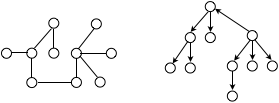
\includegraphics[scale=0.6]{FiguresGraph/tree}
       \caption{An undirected tree with 10 vertices (left) and a directed outtree (right).
       Its root is on the right upper side of the figure.}
  \label{fig:tree}
\end{center}
\end{figure}

Mathematically speaking, a tree is a graph that contains no cycles,
i.e., is {\it cycle-free}. \index{graph!cycle-free} Equivalently, a
tree is a graph in which each pair of distinct nodes is connected by
precisely one path.  A tree is thus the embodiment of ``pure''
connectivity: it provides the minimal interconnection structure that
provides paths that connect every pair of nodes.  As one might expect
from the vernacular, a set of trees is called a {\it forest}. \index{forest (of trees)}

We have just given two distinct definitions of ``tree''.  The reader
should prove that both definitions define the same class of graphs.

\begin{prop}
\label{thm:2defns-trees}
Prove that the two definitions of ``tree'' are equivalent.  In other
words, prove that the following assertions about a connected graph
$\t$ are equivalent, in the sense that one assertion holds if, and
only if, the other does.
\begin{enumerate}
\item
The graph $\t$ is cycle-free.
\item
Each pair of distinct nodes of $\t$ is connected by precisely one
path.
\item
An $n$-node connected tree $\t$ has precisely $n-1$ edges.
\end{enumerate}
\end{prop}

Let us detail the proof of the last property.

\begin{proof}
\noindent 
Let us proceed by induction on $n$.

The base case $n=2$ is obvious, because one edge is both necessary and
sufficient to connect two nodes.

Assume for induction that the indicated tally is correct for all trees
having no more than $k$ nodes.

Consider, for the purpose of extending the induction, any tree $\t$ on
$k+1$ nodes.  Easily, $\t$ must contain at least one leaf-node---i.e.,
a node $v$ of degree $1$---or else $\t$ would contain a cycle.  If we
remove $v$ and its incident edge, we now have a tree on $k$ nodes
which, by induction, has $k-1$ edges.  When we reattach node $v$, to
restore $\t$ to its original state, we see that $\t$ has $k+1$ nodes
and $k$ edges.

Because $\t$ was an arbitrary $(k+1)$-node tree, the induction is
extended.  \qed
\end{proof}

\bigskip

\noindent \fbox{
\begin{minipage}{0.95\textwidth}
Sociologically, the historical {\it atomic family tree}
\index{family tree} has two roots, representing the matriarch and patriarch of the
family.  The entirety of the tree represents a single family
generationally, before any children form their own families.  All
child-nodes in this genre of tree are the roots of singly-rooted
subtrees of the entire family tree.  The leaves of the tree are the
childless descendants of the roots.  Note that, while we are using
anthropomorphic language here, we could be discussing other genres of
``family'', as, e.g., many types of biological taxonomies.
\end{minipage}
}
\bigskip

Among rooted directed trees, an important subclass comprises those
that have a {\em single root} which has a directed path to every other
node.  The length of each such directed path is often used to label
the {\it generation}
\index{generation of a node in a singly-rooted directed tree}
of the node at the end of the path: root, child, grandchild,
great-grandchild, etc.
Every node of the tree is the root of a singly-rooted directed
subtree of the entire tree.  All subtrees that are rooted at nodes of
the same generation are mutually disjoint.
\bigskip

\noindent \fbox{
\begin{minipage}{0.95\textwidth}
A singly-rooted tree represents a {\it hierarchy}.
\index{trees!singly-rooted!hierarchy} \index{hierarchy} Given two
directed subtrees within a hierarchy, either the root of one of the
subtrees is a descendant of the root of the other, or the two subtrees
are are mutually disjoint.
\end{minipage}
}
\bigskip

More formally: {\em rooted trees} are a class of {\em acyclic}
digraphs.  Paths in trees which start at the root are often called
{\em branches}.  The {\em acyclicity} of a tree $\t$ means that for
any branch of $\t$ of the form (\ref{eq:di-path}), we cannot have $u_1
= u_n$, for this would create a cycle.  Each singly-rooted tree $\t$
has a designated {\em root node} \index{trees!root node} $u_n \in
\n_{\ft}$ that resides at the end of a branch (\ref{eq:di-path}) that
starts at $r_{\ft}$ (so $u_1 = r_{\ft}$) is said to reside at {\em
  depth} $n-1$ in $\t$; by convention, $r_{\ft}$ is said to reside at
depth $0$.  \index{depth of a node in a singly-rooted tree} $\t$'s
root $r_{\ft}$ has some number (possibly $0$) of arcs that go from
$r_{\ft}$ to its {\em children,} each of which thus resides at depth
$1$ in $\t$; in turn, each child has some number of arcs (possibly
$0$) to its children, and so on.  For each arc $(u \rightarrow v) \in
A_{\ft}$, we call $u$ a {\it parent} \index{trees!parent node} of $v$,
and $v$ a {\it child} \index{trees!child node} of $u$, in $\t$;
clearly, the depth of each child is one greater than the depth of its
parent.  Every node of $\t$ except for $r_{\ft}$ has precisely one
parent; $r_{\ft}$ has no parents.  A childless node of a tree is a
{\em leaf}, \index{trees!leaf node} i.e., a node of degree $1$.  The
transitive extensions of the parent and child relations are,
respectively, the {\em ancestor} \index{trees!ancestor node} and {\em
  descendant} \index{trees!descendant node} relations.  The {\em
  degree} \index{degree (of a node in a tree)} of a node $v$ in a tree
is the number of children that the node has, call it $c_v$.  If every
non-leaf node in a tree has the same degree $c$, then we call $c$ the
{\em degree of the tree}.  \index{degree of a tree}

It is sometimes useful to have a symbolic notation for the ancestor
and descendant relations.  To this end, we write $(u \Rightarrow v)$
\index{$\Rightarrow$: ancestor/descendant in a rooted tree} to
indicate that node $u$ is an {\it ancestor} of node $v$, or
equivalently, that node $v$ is a {\it descendant} of node $u$.  If we
decide that we are not interested in {\em really distant} descendants
of the root of a tree $\t$, then we can {\em truncate} \index{truncated}
$\t$ at a desired depth $d$ by removing all nodes whose depths exceed
$d$.  We thereby obtain the {\em depth-$d$ prefix} of $\t$.

\ignore{****************
Figure \ref{fig.graph-samples} depicts an arc-labeled rooted tree $\t$
whose arc labels come from the alphabet $\{a,b\}$.  $\t$'s arc-induced
relationships are listed in Table~\ref{tab.graph-samples}.
\begin{figure}[htb]
\centerline{\epsfig{figure=graph.sample.eps,height=4truecm}}
\caption{An arc-labeled rooted tree $\t$ whose arc labels come from
  the alphabet $\{a,b\}$.  (Arc labels have no meaning; they are just
  for illustration.)
\label{fig.graph-samples}}
\end{figure}
\begin{table}[htb]
{\small
\begin{center}
\fbox{
\begin{tabular}{c||c|c|c|c}
\multicolumn{5}{c}{The arc-labeled rooted tree $\t$ of
  Figure \ref{fig.graph-samples}} \\
\hline
Node            & Children & Parent & Descendants & Ancestors \\
\hline
\hline
$r_{\ft} = u_0$ 
& $u_1$
& none & 
$u_1, u_2, \ldots, u_k, v_1, v_2, \ldots, v_k,
w_1, w_2, \ldots, w_k$
& none \\
\hline
$u_1$
& $u_2, v_1$
& $u_0$ & 
$u_2, \ldots, u_k, v_1, v_2, \ldots, v_k, w_1, w_2, \ldots, w_k$
& $u_0$ \\
\hline
$u_2$
& $u_3, v_2$
& $u_1$ & 
$u_3, \ldots, u_k, v_2, \ldots, v_k, w_2, \ldots, w_k$
& $u_0$ \\
\hline
 $\vdots$ & $\vdots$ & $\vdots$ &  $\vdots$ &  $\vdots$ \\
\hline
$u_k$
& $v_k$ 
& $u_{k-1}$ & 
$v_k, w_k$
& $u_0, u_1, \ldots, u_{k-1}$ \\
\hline
$v_1$
& $w_1$ 
& $u_1$ & 
$w_1$
& $u_0, u_1$ \\
\hline
$v_2$
& $w_2$
& $u_2$ & 
$w_2$
& $u_0, u_1, u_2$ \\
\hline
 $\vdots$ & $\vdots$ & $\vdots$ &  $\vdots$ &  $\vdots$ \\
\hline
$v_k$
& $w_k$
& $u_k$ & 
$w_k$
& $u_0, u_1, \ldots, u_k$ \\
\hline
$w_1$
& none
& $v_1$ & 
none
& $u_0, u_1, v_1$ \\
\hline
$w_2$
& none &
$v_2$ & 
none
& $u_0, u_1, u_2, v_2$ \\
\hline
$w_k$
& none
& $v_k$ & 
none
& $u_0, u_1, \ldots, u_k, v_k$
\end{tabular}
}
\end{center}
}
\caption{A tabular description of the rooted tree $\t$ of
  Figure \ref{fig.graph-samples}.  \label{tab.graph-samples}}
\end{table}
*********************}

\noindent{\it Spanning trees}.
One of the major uses of trees and forests is as a way of succinctly
``summarizing'' the connectivity structure inherent in an undirected
graph.  This role is inherent in the notion of a {\it spanning tree}
\index{graph!spanning tree} \index{spanning tree} \index{tree!spanning tree}
of a connected graph $\g$.  A spanning tree of $\g$ is a tree $\t(\g)$
whose node-set is identical to $\g$'s:
\[ \n_{\ft(\fg)} \ = \ \n_{\fg} \]
and all of whose edges are edges of $\g$:
\[ \e_{\ft(\fg)} \ \subseteq \ \e_{\fg}. \]
Not surprisingly, a connected graph $\g$  typically has {\em many}
spanning trees.  All such trees share $\g$'s node-set, but they may
choose quite different sets of edges.

\ignore{***

For a graph $\g$ that is not connected, we replace the notion of
spanning tree of $\g$ with the analogous notion of a {\it spanning
  forest} \index{graph!spanning forest} \index{spanning forest} of
$\g$.  We shall typically discuss only spanning trees in this section,
leaving the reader to extrapolate the discussion to include spanning
forests of unconnected graphs.
***}


The major use of spanning trees in applications is to ``summarize''
the full connectivity structure of a graph---and of the entities that
the graph models, such as a map, the layout of a museum, etc.  When
used in this way, the edges of spanning trees are typically {\em
  weighted}, \index{graph!spanning tree!edge-weighted} in order to
model a ``cost'' of incorporating that edge in the tree.  The types of
computational problem modeled via edge-weighted spanning trees
include: the optimal placement of firehouses, or hospitals, in a town
and the optimal deployment of security mechanisms in an art museum.
Reflecting problems wherein edge-weights measure transit costs, it is
a classical computational problem to seek a {\em minimum-weight
  spanning tree} \index{graph!minimum-weight spanning tree}
\index{minimum-weight spanning tree} (or, in the vernacular, a {\em
  minimum spanning tree}).  Happily, this classical optimization
problem can be solved within a number of steps that is linear in the
number of edges of $\g$ \cite{CLRS}.

\ignore{*****
I put in the exercice session
{\Arny Giving just a {\em hint} at a solution for MST to real
  beginners is probably useless}

There are mainly two ways for constructing such a MST, each one
emphasizes a different propriety of the MST, namely, avoid cycles and
minimize the span.  In both cases, the edges are sorted in increasing
order of weights.  More precisely, the first one constructs a subtree
which partially spans the graph by adding at each step the minimum
neighboring edge while the other add successively the edges of minimal
weights that do not create a cycle.
****}

Just as with graphs, there is a {\em directed} version of trees which
is formed by replacing the (unoriented) edges of an undirected tree by
(oriented) arcs; see the right side of Fig.~\ref{fig:tree}.  Within a directed tree
$\t$, one often says that an arc goes from a {\it parent node}
\index{trees!parent node} to a {\it child node}
\index{trees!child node}.  Extending this anthropomorphic metaphor, one often talks
about the {\it ancestor(s)} \index{trees!ancestor node} and {\it
  descendant(s)} \index{trees!descendant node} of a tree-node.  We
single out two special classes of nodes: A {\it root (node)}
\index{trees!root (node)} \index{root (of a directed tree)} of $\t$ is
defined by its having no entering arcs, i.e., indegree $0$; a {\it
  leaf (node)} \index{trees!leaf (node)} 
\index{leaf (of a directed tree)} of $\t$ is defined by its having no
exiting arcs, i.e., outdegree $0$.  The reader is certainly familiar
with the use of rooted directed trees to represent family trees and
corporate hierarchies.

%%%%%%%%%%%%%%%%%%%%%%%%%%%%%%%%%%%

\section{Computationally Significant ``Named'' Graphs}
\label{sec:graphs-important-families}

The mathematical discipline called graph theory is an important source
of formal aids for the activities of designing, analyzing, utilizing,
and verifying computer systems.  Of course, computer systems are
designed by humans.  Among other consequences of this fact is the
observations that the graphs that are among the most commonly used to
structure systems tend to be rather uniform in structure, in a variety
of possible ways.  Such graphs, when drawn, often exhibit a lot of
structural symmetry.  One popular form of symmetry is {\it degree
  regularity}: an undirected graph $\g$ is {\it regular}
\index{graph!regular} if all nodes of $\g$ have the same degree.  Not
surprisingly, there is a directed version of ``regular'' embodied in the
symmetric notions of {\it in-regularity}
\index{graph!directed!in-regular} and {\it out-regularity}.
\index{graph!directed!out-regular}

\medskip

We now describe five families of regular graphs that have proven
useful over the history of digital computing, and we expose some basic
properties of each, including its diameter.  Each of these graphs is
available in both a directed and an undirected version, although, as
we note, one of these versions is more commonly encountered.  We have
selected these specific graphs for rather different reasons.
\begin{itemize}
\item
The first two graphs, the {\it cycle-graph} of Section~\ref{sec:cycle}
and the {\it complete graph} of Section~\ref{sec:clique} were selected
for representing, respectively, the lowest-degree and highest-degree
graphs that share two properties: (1) every node of each graph is
accessible from every other node; (2) all nodes ``look alike'' to
someone traversing the graph.  Elaborating on (2): If we put you down
on a node of either graph, there is no way that you can determine the
identity of that node.  This is an important feature to ponder,
because it is a simple instance of the anonymity problem inherent to
many modern distributed computing environments.  {\it How does one
  orchestrate cooperative activities when all agents ``are
  identical''?}
\item
The remaining graphs, the {\it mesh and torus networks}\footnote{These
  two structures, though distinct, are usually discussed together
  because they share so many important properties.}~of~\ref{sec:mesh},
the {\it hypercube network} of Section~\ref{sec:hypercube}, and the
{\it de Bruijn network} of Section~\ref{sec:deBruijn}, were selected
for their importance within the world of parallel and distributed
computing---as abstract platforms for developing efficient
computational and communicational processes, and as abstract versions
of the networks that underlie parallel architectures by
interconnecting its processors.
\end{itemize}
Throughout, the parameters that describe our graph families range over
the positive integers; i.e., each occurrence of $n$ below ranges over
$\N^+$.

\subsection{The {\it Cycle-graph} $\cc_n$}
\label{sec:cycle}

{\Denis The notation with a hat for the directed version is not the same as
the reverse graph presented before. Do we really need to present the reverse graph???}

For each positive integer $n \in \N^+$, both the {\it undirected
  order-$n$ cycle-graph} $\cc_n$ and the {\it directed order-$n$
  cycle-graph} $\widehat{\cc}_n$ \index{cycle graph}
\index{cycle network} have {\it node-set}
\[ \n_{{\cal C}_n} \ = \ \n_{\widehat{{\cal C}}_n}
\ = \ \{ 0, \ 1, \ \ldots, \ n-1\}. \]
\begin{itemize}
\item
$\cc_n$ has $n$ edges; its {\it edge-set} is
\[ \e_{{\cal C}_n} \ = \
\big\{ \{i, \ i+1 \bmod n\} \ \ | \ \ i \in \{0, \ 1, \ \ldots,
\ n-1\} \big\}.
\]
Fig.~\ref{fig:cycle} illustrates a cycle with $8$ vertices.
  \begin{itemize}
  \item \index{cycle graph!node-degree}
$\cc_n$ is a regular network: each node has degree $2$.

Specifically, each node $i$ of $\cc_n$ has its {\it predecessor} $i-1
\bmod n$ \index{cycle graph!predecessor node}
\index{cycle graph!successor node} and its {\it successor} $i+1 \bmod n$ .
  \item \index{cycle graph!diameter}
$\cc_n$ has diameter $\lfloor n/2 \rfloor$.

Direct calculation shows that $\cc_n$'s diameter is no larger than
this.  The fact that this is, in fact, the graphs's diameter is
witnessed by the distance between each node $k \in \n_{{\cal C}_n}$
and its antipodal node $k + \lfloor n/2 \rfloor \bmod n$.
  \end{itemize}

\item
$\widehat{\cc}_n$ has {\it arc-set}
\[ \a_{\widehat{{\cal C}}_n} \ = \ 
\big\{ (i \rightarrow i+1 \bmod n) \ \ | \ \ i \in \{0, \ 1, \ \ldots, \ n-1\} \big\}
\]
  \begin{itemize}
  \item \index{cycle graph!directed node-degree}
$\widehat{\cc}_n$ is a regular network: each node has the same
    indegree and the same outdegree.  Coincidentally, both the common
    indegree and the common outdegree are $2$.
  \item
$\widehat{\cc}_n$ has (directed) diameter $n-1$.

Of course, $n-1$ is an upper bound on the diameter of any $n$-node
digraph.  The fact that this is exactly the graph's diameter is
witnessed by the directed distance from each node $k$ of $\widehat
{\cc}_n$ to its predecessor node $k-1 \bmod n$.
  \end{itemize}
\end{itemize}

\begin{figure}[hbt]
\begin{center}
       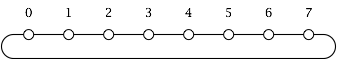
\includegraphics[scale=0.6]{FiguresGraph/cycle}
       \caption{A cycle of $8$ vertices.}
  \label{fig:cycle}
\end{center}
\end{figure}

\subsection{The {\it Complete graph}, or, {\it Clique} $\k_n$}
\label{sec:clique}
\index{complete graph} \index{clique}

For each positive integer $n \in \N^+$, we denote by $\k_n$ the {\em
  undirected} order-$n$ {\it complete-graph} (or, {\it clique}),
\index{complete graph} \index{clique} and by $\widehat{\k}_n$ the {\em
  directed} order-$n$ {\it complete-graph} (or, {\it clique}).  Both
$\k_n$ and $\widehat{\k}_n$ have {\it node-set}
\[ \n_{{\cal K}_n} \ = \ \n_{\widehat{{\cal K}}_n}
\ = \ \{ 0, \ 1, \ \ldots, \ n-1\}. \]
\begin{itemize}
\item
$\k_n$ has $\displaystyle {n \choose 2}$ edges; its {\it edge-set} is
\[ \e_{{\cal K}_n} \ = \
\big\{ \{i, \ j\} \ \ | \ \ i,j \in \{0, \ 1, \ \ldots, \ n-1\}, \ i
\neq j \big\}.
\]
  \begin{itemize}
  \item \index{complete graph!node-degrees} \index{clique!node-degrees}
$\k_n$ is a regular network: each node has degree $n-1$; every node $i
\in \n_{\fk_n}$ is connected with all other nodes.

   \item \index{complete graph!diameter}
$\k_n$ has diameter $1$.

$\k_n$'s diameter is a direct consequence of its node-degrees, and vice versa.
  \end{itemize}

\item
$\widehat{\k}_n$ has $(n-1)n$ arcs; its {\it arc-set} is
\[ \a_{\widehat{{\cal K}}_n} \ = \ 
\big\{ (i \rightarrow j) \ \ | \ \ i,j \in \{0, \ 1, \ \ldots, \ n-1\}
\big\}, \ i \neq j
\]
  \begin{itemize}
  \item
$\widehat{\k}_n$ is a regular network: each node has the same indegree
    and the same outdegree.  Both the common indegree and the common
    outdegree are $n-1$.
  \item
$\widehat{\k}_n$ has (directed) diameter $1$.

As in the undirected case, there is a causal relationship between
$\widehat{\k}_n$'s diameter and its (in- and out-) node-degrees.
  \end{itemize}
\end{itemize}

{\Denis good opportunity for an exercice here: a tournoiment 
is a directed version of a complete graph (any orientation of the edges).
The proof that it is hamiltonian is nice, If you agree I can add it in the exercices...}

Hearkening back to our discussion of matchings in (unweighted) graphs:
The structure of the set of perfect matchings in general graphs is
decidely nontrivial.  For clique-graphs, though, the structure is much
easier to discuss.

\begin{prop}
\label{thm:perfect-matchings-clique}
The number of perfect matchings admitted by the clique-graph $\k_n$ is
either $0$---if $n$ is odd---or exponential in $n$ if $n$ is even.
\end{prop}

\begin{proof}
The assertion about cliques with odd numbers of nodes is immediate
from Proposition~\ref{thm:necessary-for-perfect-matching}.

We verify the assertion about cliques of the form $\k_{2k}$ by
induction on $k$.  To this end, let $M_n$ denote the number of perfect
matchings that the clique $\k_n$ admits.

The base of our induction is the case $k=1$.  Because $\k_{2}$
consists of a single edge, it admits only one perfect matching; i.e.,
$M_1 = 1$.
%(see Figure~\ref{perfectMatching1}): 

To garner intuition, we also explicitly solve the case $k=2$, which is
illustrated in Fig.~\ref{fig:AllPerfectMatchings}.
\begin{figure}[hbt]
\begin{center}
       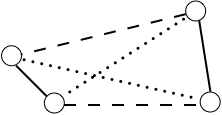
\includegraphics[scale=0.55]{FiguresGraph/perfectmatchingAll}
       \caption{The $4$-nodes Clique graph  $\k_4$ (left) and its three different perfect matchings (right): 
       the matchings' edges are drawn, respectively, with bold lines, dashed lines, and dotted lines.}
  \label{fig:AllPerfectMatchings}
\end{center}
\end{figure}
As the figure illustrates, $\k_4 = \k_{2 \cdot 2}$ can be viewed as a
$4$-cycle (drawn with bold and dashed lines), augmented by two
``cross-edges'' (drawn with dotted lines).  Easily, then, $\k_4$
admits $3$ different perfect matchings, which can be identified (and
specified) by the edge that contains the northwesterly node---call it
$v$---in the figure.  Node $v$ has the choice of three nodes to
``boldly'' match with. (In the figure, $v$ has chosen the
southwesterly node as its ``bold'' match.)  Once $v$ has chosen its
match, there is only one viable choice for the second edge in the
matching.  Thus, $M_2=3$.

We jump now to the case of any arbitrary $k > 2$.  We remark that
there are precisely $2k-1$ nodes of $\k_{2k}$ that node $1$ can
``choose'' as its mate in a perfect matching.  Once we set node $1$
and its chosen mate aside, we confront an independent instance of the
problem with parameter $k-1$, i.e., the problem of counting the number
of perfect matchings in $\k_{n-2} = \k_{2k-2}$.  We thereby note that
as $k$ grows, the quantity $M_k$ obeys the following recurrence:
\[ M_k \ = \ (2k-1) \cdot M_{k-1} \]
In other words:

\hspace*{.25in}{\em $M_k$ is the product of the first $k$ odd numbers.}
%$N_1=1$, $N_2=3$, $N_3=3 \times 5=15$, $N_4=3 \times 5 \times 7=115$, etc..

\noindent
To gauge the growth rate of $M_k$, we concentrate on cases $k > 2$ and
ignore the $\lfloor k/2 \rfloor$ smallest odd numbers.  We then
replace each of the remaining odd numbers by its smallest possible
value.  We thereby find that
\[
M_k \ \ =    \ \ \prod_{i=1}^k \ (2i-1)
    \ \ \geq \ \ \prod_{\lceil k/2 \rceil}^k \ (2i-1)
    \ \ \geq \ \ \left( 2 \lceil k/2 \rceil -1 \right)^{k/2}
    \ \ >    \ \ k^{k/2}
\]
In summary, $M_k$ grows exponentially with the parameter $k$, as claimed.
\qed
\end{proof}


\bigskip

The two families of graphs we have just discussed, cycles and cliques,
are recommended to our attention by their structural simplicity---they
epitomize, respectively, the most sparse way (the cycle) and the most
dense way (the clique) to completely interconnect $n$ nodes.  The
remainder of this section is devoted to three graph-structures that
are structurally more complex than cycles and cliques, which have been
designed to meet specific needs within the real technological world of
computing and communicating.  Indeed, the three upcoming graph
families are among the most important ones when discussing parallel
and distributed computing (PDC, for short).  All three families have
been used both to design computer architectures that support PDC and
to craft algorithms that exploit the potential efficiencies---in
computation and communication---that one can achieve using PDC.

\subsection{Sibling networks: the {\it M}esh ($\m_{m,n}$) and the {\it Torus} ($\widetilde{\m}_{m,n}$)}
\label{sec:mesh}
\index{mesh and torus networks}

For positive integers $m, n \in \N^+$, both the $m \times n$ {\it mesh
  (network)} $\m_{m,n}$ and the $m \times n$ {\it toroidal network}
(or, {\it torus}) $\widetilde{\m}_{m,n}$ have {\it node-set}
\begin{eqnarray*}
\n_{\fm_{m,n}} \ = \ \n_{\widetilde{\fm}_{m,n}}
  & = & 
\{1, \ 2, \ldots, \ m\} \ \times \ \{1, \ 2, \ldots, \ n\} \\
  & = & 
\big\{ \langle i, \ j \rangle \ \ | \ \ 
\big[ i \in \{1, \ 2, \ldots, \ m\} \big], \ \
\big[ j \in \{1, \ 2, \ldots, \ n\} \big]
\big\}
\end{eqnarray*}

\begin{itemize}
\item
$\m_{m,n}$ has $(m-1)n \ + \ (n-1)m$ edges; its {\it edge-set} is
\begin{eqnarray*}
\e_{\fm_{m,n}} & = & 
\big\{
\{ \{ i, j \}, \ \{ i+1, j \} \ \ | \ \
1 \leq i < m, \ \ 1 \leq j \leq n \} \\
  &  & \hspace*{.1in} \cup
\{ \{ i, j \}, \ \{ i, j+1 \} \ \ | \ \
1 \leq i \leq m, \ \ 1 \leq j < n \}
\big\}
\end{eqnarray*}

{\Denis I removed the formal definitions of corners, edges
since I don't see what this really add to the text (we don't use this later),
let discuss if you disagree... }

\begin{itemize}
\item
The subgraph of $\m_{m,n}$ defined by the node-set
\[ \{ \langle i, \ j \rangle  \ \ | \ \ \left[i \in \{1, 2, \ldots,
  m\}\right], \ \ \left[1 \leq j < n\right]\}
\]
{\Denis Definition not clear: for me, $i$ should be fixed, and then, $j$ varies}
and all edges both of whose endpoints belong to that set is called the
$i$th {\it row} of $\m_{m,n}$
\index{row of a mesh graph}\index{mesh graph!row}
Dually, the subgraph of $\m_{m,n}$ defined by the node-set
\[ \{ \langle i, \ j \rangle  \ \ | \ \ \left[j \in \{1, 2, \ldots,
  n\}\right], \ \ \left[1 \leq i < m\right] \}
\]
and all edges both of whose endpoints belong to that set is called the
$j$th {\it column} of $\m_{m,n}$.
\index{column of a mesh graph}\index{mesh graph!column}
\ignore{*********
  \begin{itemize}
     \item
Nodes $\langle 1, \ 1 \rangle$, $\langle 1, \ n \rangle$, $\langle m,
\ 1 \rangle$, and $\langle m, \ n \rangle$ are the {\it corner nodes}
(or, just {\it corners}) of $\m_{m,n}$.
\index{corner (node) of a mesh graph}
\index{mesh graph!corner (node)}
     \item
The path-graph consisting of the node-set
\[ \{ \langle 1, \ 1 \rangle, \ \langle 1, \ 2 \rangle, \ldots, \
\langle 1, \ n \rangle \}
\]
together with all edges of $\m_{m,n}$ both of whose endpoints belong
to this set, is the {\it top edge} of $\m_{m,n}$.
\index{top edge of a mesh graph}
\index{mesh graph!top edge}

The other edges of $\m_n$ are defined analogously:

\smallskip

The {\it bottom edge} of $\m_{m,n}$ is the path-graph built upon the
node-set
\[ \{ \langle m, \ 1 \rangle, \ \langle m, \ 2 \rangle, \ldots, \
\langle m, \ n \rangle \}
\]
\index{bottom edge of a mesh graph}
\index{mesh graph!bottom edge}

The {\it left edge} of $\m_{m,n}$ is the path-graph built upon the
node-set
\[ \{ \langle 1, \ 1 \rangle, \ \langle 2, \ 1 \rangle, \ldots, \
\langle m, \ 1 \rangle \}
\]
\index{left edge of a mesh graph}
\index{mesh graph!left edge}

The {\it right edge} of $\m_{m,n}$ is the path-graph built upon the
node-set
\[ \{ \langle 1, \ n \rangle, \ \langle 2, \ n \rangle, \ldots, \
\langle m, \ n \rangle \}
\]
\index{left edge of a mesh graph}
\index{mesh graph!right edge}
     \end{itemize}
********}

  \item 
$\m_{m,n}$ is {\em not} a regular graph.  Its four corner nodes each has
    degree $2$; its non-corner extreme edge nodes each has degree $3$; its
\index{mesh graph!node-degree}\index{internal node of a mesh graph}
\index{mesh graph!internal node}
{\em internal nodes} each has degree $4$

  \item \index{mesh graph!undirected diameter}
The diameter of $\m_{m,n}$ is $m+n-2$, as witnessed by the distance
between nodes $\langle 1, \ 1 \rangle$ and $\langle 2, \ n \rangle$.
  \end{itemize}

\item
$\widetilde{\m}_{m,n}$ has $2mn$ arcs; its {\it arc-set} is
\begin{eqnarray*}
\a_{\widetilde{\m}_{m,n}} & = &
\big\{
\{ (\langle i, \ j \rangle \rightarrow \langle i+1 \bmod m, \ j
\rangle) \ \ | \ \ 1 \leq i \leq m, \ \ 1 \leq j \leq n \} \\
  &  & \hspace*{.1in} \cup
\{ (\langle i, \ j \rangle \rightarrow \langle i, \ j+1 \bmod n
\rangle) \ \ | \ \ 1 \leq i \leq m, \ \ 1 \leq j \leq n \}
\big \}
\end{eqnarray*}

\ignore{***********
  \begin{itemize}
  \item
The subgraph of $\widetilde{\m}_{m,n}$ defined by the node-set
\[ \{ \langle i, \ j \rangle  \ \ | \ \ \left[i \in \{1, 2, \ldots,
  m\}\right], \ \ \left[1 \leq j \leq n\right]\}
\]
and all edges both of whose endpoints belong to that set is called the
$i$th {\it row} of $\widetilde{\m}_{m,n}$
\index{torus graph!row}
Dually, the subgraph of$\widetilde{\m}_{m,n}$ defined by the node-set
\[ \{ \langle i, \ j \rangle  \ \ | \ \ \left[j \in \{1, 2, \ldots,
  n\}\right], \ \ \left[1 \leq i \leq m\right] \}
\]
and all edges both of whose endpoints belong to that set is called the
$j$th {\it column} of $\widetilde{\m}_{m,n}$.
\index{torus graph!column}
**********}
\begin{itemize}
  \item
$\widetilde{\m}_{m,n}$ is a regular network; each node has degree $4$.
    Despite the fact that $\widetilde{\m}_{m,n}$ is an {\em
      undirected} graph, its arcs are commonly referred to via an
    anthropomorphic labeling, either as ``up, down, left, and right''
    or as ``north, south, west, and east''.
  \item \index{mesh graph!directed diameter}
$\widetilde{\m}_{m,n}$'s diameter is $\lfloor m/2 \rfloor \ + \
\lfloor n/2 \rfloor$.  This can be verified in analogy to the diameter
of the cycle-graph $\cc_n$.
\end{itemize}
\end{itemize}

\begin{figure}[hbt]
\begin{center}
       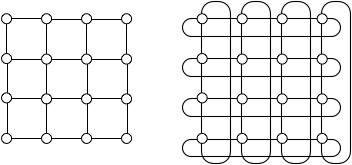
\includegraphics[scale=0.6]{FiguresGraph/meshtorus}
       \caption{$\m_{4,4}$ (left) and $\widetilde{\m}_{4,4}$ (right).}
  \label{fig:torus}
\end{center}
\end{figure}

\subsection{The (Boolean) {\it Hypercube} $\q_n$}
\label{sec:hypercube}
\index{boolean hypercube}
\index{hypercube}

The graphs we focus on in this section have had a major impact on the
world of coding, especially in regard to codes that are {\em error
  correcting} \cite{PetersonW81}, and the world of computing,
especially in regard to parallel and distributed computing
\cite{JohnssonH1989, SaadS89, Schwartz80}.  The cited sources give a
range of perspectives on the importance of {\it hypercube networks.}

\index{order-$n$ boolean hypercube}
The {\it order-$n$ boolean hypercube}, traditionally denoted $\q_n$,
is the $2^n$-node graph defined as follows.
\begin{itemize}
\item
{\it The recursive definition}. 
\index{order-$n$ boolean hypercube!recursive definition}
  \begin{itemize}
  \item
The order-$0$ boolean hypercube, $\q_0$, has a single node, and no
edges.
  \item
The order-$(k+1)$ boolean hypercube, $\q_{k+1}$, is obtained by taking
two copies of $\q_k$, call them $\q_k^{(1)}$ and $\q_k^{(2)}$, and
creating an edge that connects each node of $\q_k^{(1)}$ with the
corresponding node of $\q_k^{(2)}$.
  \end{itemize}
For illustration:
  \begin{itemize}
  \item
$\q_1$ consists of two nodes connected by a single edge.
  \item
$\q_2$ can be viewed as a ``square'', or equivalently, a copy of $\cc_4$.
  \item
$\q_3$ can be viewed as a ``cube'', i.e., as two copies of $\cc_4$
    with edges connecting corresponding nodes: Each of the following
    pairs of nodes are connected by an edge: the upper right
    corner-nodes, the upper left corner-nodes, the lower right
    corner-nodes, and the lower left corner-nodes.
  \end{itemize}

\item
{\it The direct definition}.
For each $n \in \N$, the nodes of the order-$n$ boolean hypercube,
$\q_n$, are all length-$n$ binary strings.  For illustration:
\index{order-$n$ boolean hypercube!direct definition}
\begin{eqnarray*}
\n_{{\fq}_0}
  & = & 
\{ \varepsilon \}, \ \ \mbox{ the length-$0$ {\em null string}} \\ 
\n_{{\fq}_1}
  & = &
\{ 0, \ 1 \} \\
\n_{{\fq}_2}
  & = & \{ 00, \ 01, \ 10, \ 11 \} \\
\n_{{\fq}_3}
  & = & \{ 000, \ 001, \ 010, \ 011, \ 100, \ 101, \ 110, \ 111 \} 
\end{eqnarray*}
The iteration-based construction of big hypercubes from the next
smaller ones is illusrated in Fig.~\ref{fig:hypercube}.
\begin{figure}[hbt]
\begin{center}
       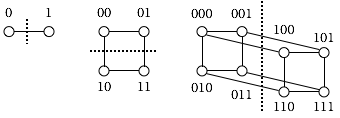
\includegraphics[scale=0.6]{FiguresGraph/hypercube}
\caption{The iteration-based construction of order-$n$ hypercubes:
  Take two copies of the order-$(n-1)$ hypercube.  Prepend a $0$ to
  the node-labels of the first copy and a $1$ to the node-labels of
  the second copy.}
  \label{fig:hypercube}
\end{center}
\end{figure}

Easily, for each value of $n$, $\q_n$ has $2^n$ nodes, for this is the
number of length-$n$ binary strings.

\medskip

For each value of $n$, each edge of $\q_n$ connects two node-strings
that differ in precisely one position.  This means that $\q_n$ has $n
2^{n-1}$ edges: To wit, each of its $2^n$ nodes has $n$ neighbors, so
the quantity $n 2^n$ counts each of $\q_n$'s edges twice---one for
each endpoint.  For illustration:
\begin{eqnarray*}
\e_{{\fq}_1}
  & = &
\big\{ \{ 0, \ 1 \} \big\} \\
\e_{{\fq}_2}
  & = & \big\{
\{ 00, \ 01 \}, \ \{ 00, \ 10\}, \
\{ 01, \ 11 \}, \ \{ 10, \ 11\} 
\big\} \\
\e_{{\fq}_3}
  & = & \big\{ 
\{000, \ 001\}, \
\{000, \ 010\}, \
\{000, \ 100\}, \
\{001, \ 011\}, \\
  &  & \hspace*{.2in}
\{001, \ 101\}, \
\{010, \ 011\}, \
\{010, \ 110\}, \
\{100, \ 101\}, \\
  &  & \hspace*{.2in}
\{100, \ 110\}, \
\{101, \ 111\}, \
\{011, \ 111\}, \
\{110, \ 111\}
\big\}
\end{eqnarray*}
\end{itemize}

\medskip

\noindent
It is easy to observe $\q_n$'s basic structural properties.
\begin{itemize}
\item \index{hypercube!node-degree}
$\q_n$ is a regular network: each of its $2^n$ nodes has degree $n$.

This follows from the fact that each edge of $\q_n$ rewrites a single
bit-position in the length-$n$ binary string that is the edge's source
node.

\item \index{hypercube!diameter}
$\q_n$ has diameter $n \ = \ \ln(|\n_{\fq_n}|)$.\footnote{Recall that
  $\ln n = \log_2 n$; see Section~\ref{sec:exponential+logarithm}.}

We address this issue formally.
\end{itemize}

\begin{prop}
\label{thm:hypercube-diameter}
For all $n \in \N^+$, $\q_n$ has diameter $n \ = \ \ln(|\n_{\fq_n}|)$.
\end{prop}

\begin{proof}
We prove this diameter bound by construction.  Focus on two arbitrary
nodes of $\q_n$:
\[ x \ = \ \alpha_1 \alpha_2 \cdots \alpha_n \ \ \ \mbox{ and } \ \ \
y \ = \ \beta_1 \beta_2 \cdots \beta_n
\]
One of the several paths in $\q_n$ from $x$ to $y$ is described
schematically as the following left-to-right, bit-by-bit rewriting of
$x$ as $y$ using edges of $\q_n$
\[
x \ = \ \alpha_1 \alpha_2 \cdots \alpha_n \ \rightarrow \
\beta_1 \alpha_2 \cdots \alpha_n \ \rightarrow \
\beta_1 \beta_2\cdots \alpha_n \ \rightarrow \cdots \rightarrow\ 
\beta_1 \beta_2 \cdots \beta_n \ = \ y
\]
Since each bit of each string is rewritten at most once (only if $\alpha_i \neq \beta_i$), the bound follows.
\qed
\end{proof}

\medskip

The fact that $\q_n$'s diameter is {\em logarithmic} in its size makes
$\q_n$ an efficient network for many tasks related to parallel
computing and communication.
\bigskip

A powerful avenue for understanding the structure of a given family of
networks is to understand how the perceived ``shape'' of graphs in the
family can apparently change just by relabeling/renaming the nodes, or
the edges, of the graphs.  The formal mechanism for studying such
relabelings/renamings is the concept of {\it graph isomorphism}.
\index{graph isomorphism} Let $\g$ and $\h$ be undirected graphs that
have the same numbers of nodes and edges.  (The following definition
can easily be adapted to deal with {\em directed} graphs.)  An {\it
  isomorphism} between $\g$ and $\h$ is a {\em
  bijection}\footnote{Recall, from Chapter~\ref{ch:sets-BA-logic} that
  a bijection is a function that is one-to-one (i.e., injective) and
  onto (i.e., surjective).}
\[ f: \n_{\fg} \ \leftrightarrow \ \n_{\fh} \]
such that
\begin{itemize}
\item
For each edge $\{ u,v \}$ of $\g$ (i.e., $\{ u,v \} \in \e_{\fg}$),
the doubleton set $\{ f(u), f(v) \}$ is an edge of $\h$ (i.e.,
$\{ f(u), f(v) \} \in \e_{\fh}$).
\item
For each edge $\{ x,y \}$ of $\h$ (i.e., $\{ x,y \} \in \e_{\fh}$),
the doubleton set $\{ f^{-1}(x), f^{-1}(y) \}$ is an edge of $\g$ (i.e.,
$\{ f^{-1}(x), f^{-1}(y) \} \in \e_{\fg}$).
\end{itemize}
We can immediately exemplify this notion via the following example.

\begin{prop}
The order-$4$ hypercube $\q_4$ is \textit{isomorphic} to the $4 \times
4$ torus $\widetilde{\m}_{4,4}$.
\end{prop}

\begin{figure}[hbt]
\begin{center}
       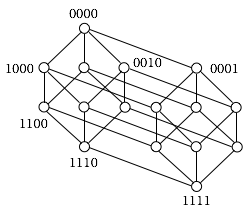
\includegraphics[scale=0.6]{FiguresGraph/Isomorphism1}
       \caption{A representation of $\q_4$ with partial coding of the vertices.}
  \label{fig:isomorphism1}
\end{center}
\end{figure}

\begin{figure}[hbt]
\begin{center}
       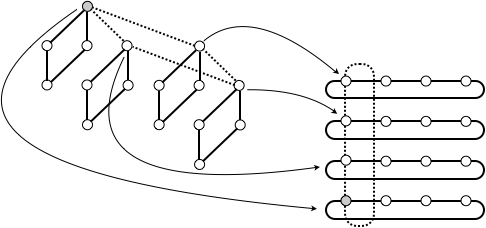
\includegraphics[scale=0.5]{FiguresGraph/Isomorphism2}
       \caption{Transformation of $\q_4$ to a $4 \times 4$ torus.
       The bold edges correspond to the horizontal cycles and the dashed edges correspond to vertical cycles.}
  \label{fig:isomorphism2}
\end{center}
\end{figure}

A graphical proof is depicted in Fig.~\ref{fig:isomorphism1}  and ~\ref{fig:isomorphism2} and 
We relegate the formal proof of this result to a Exercise
{\Denis add a ref here?}, supplying as a
hint the coding scheme (or, bijection) depicted in
Fig.~\ref{fig:toruslabel}.
\begin{figure}[hbt]
\begin{center}
       \includegraphics[scale=0.6]{FiguresGraph/toruslabel}
\caption{Sketching the coding scheme that yields an isomorphism
  between the order-$4$ hypercube $\q_4$ and the $4 \times                          
4$ torus $\widetilde{\m}_{4,4}$.}
  \label{fig:toruslabel}
\end{center}
\end{figure}


\subsection{The {\it de Bruijn} network $\d_n$}
\label{sec:deBruijn}
\index{de Bruijn network}
\index{de Bruijn graph}

While the family of hypercube networks has few competitors in the
world of parallel and distributed computing, in terms of performance
and ease of designing algorithms, it does have one major shortcoming
that relates to its realizability in hardware.  The basic problem is that each node of the
order-$n$ hypercube has node-degree $n$; i.e., the node-degrees are logarithmic
in the size of the network.  This feature makes the hypercube's actual
performance much slower than its theoretical performance: each step of a node $v$ of $\q_n$ is slowed down by $v$'s having
to get inputs from and supply outputs to its $n$ (directed) neighbors.  The phenomenon we are discussing can actually
be described {\em geographically}!  The physical area that an order-$n$ hypercube $\q_n$ occupies grows
{\em exponentially} with the
common degrees of the network's nodes---because $\q_n$ has $2^n$ nodes which are no more than $n$ 
edge-traversals from one another.  (This is the ``inverse'' way
of talking about logarithmic node-degrees.)  In contrast, the space in which we (and our computers) live grows only 
{\em cubically} with linear distance.  The resulting disparity means that the wires in large hypercube-connected
computing platforms must inevitably be very long---in contrast to the unit-size
of idealized network-edges.  Consequently, electrical signals within a
large hypercube must travel long distances in physical space---which means that the
physical computer is much slower than its idealized version.  (One
finds a more technical discussion of this phenomenon in, say, \cite{Ullman84}.)

The preceding shortcoming of hypercubes has led researchers since the 1970s to seek a
family of networks whose node-degrees stay constant even as one
deploys successively larger instances of the network.  The candidate
such network which we are currently focusing on was discovered within the domain of {\it coding theory} (as,
coincidentally, was the hypercube).  

In the mid-20-century, Dutch mathematician Nicolaas Govert de Bruijn
\index{de Bruijn, Nicolaas Govert} discovered a way to generate
compact sequences that contain all possible strings of a prespecified
length.  Focusing on {\em binary} strings---although de Bruijn's
strategy works for any finite alphabet---de Bruijn could generate a
string of length $2^n +n-1$ that contains every length-$n$ binary
string as a substring.  Quite appropriately, such a string is called a
{\it de Bruijn sequence}. \index{de Bruijn sequence} It is not obvious
that de Bruijn sequences exist for every $n$, but we now plant the
seeds of a proof that they do.  We begin by illustrating two sample
sequences in (\ref{eqn:deBruijn-seq}).
\begin{equation}
\label{eqn:deBruijn-seq}
\begin{array}{|l||c|c|}
\hline
n & \mbox{\sc Length-$n$ binary strings}
    & \mbox{\sc Order-$n$ de Bruijn sequence} \\
\hline
\hline
1 &
00, \ 01, \ 10, \ 11  & 00110 \\
\hline
2 &
\begin{array}{l}
000, \ 001, \ 010, \ 011, \\
100, \ 101, \ 110, \ 111 
\end{array}
  & 0001110100 \\
\hline
\end{array}
\end{equation}
The table in (\ref{eqn:deBruijn-seq}) spawns several interesting
questions:
\begin{itemize}
\item
Do de Bruijn sequences exist for every $n$?
\item
If so, 
  \begin{itemize}
  \item
How does one compute them?
  \item
Can one always find a de Bruijn sequence of length $2^n +n-1$?
  \item
Can one find de Bruijn sequences of length $< 2^n +n-1$?
  \end{itemize}
 \ignore{\Arny (SOME GOOD EXERCISES HERE)} 
\end{itemize}
The answers to all of these questions---and the connection of de
Bruijn sequences to the current chapter---reside in the family of
directed graphs called {\it de Bruijn graphs} (or, {\it networks}).
\index{de Bruijn graph} \index{de Bruijn network} (The term used
varies by intended application---mainly, coding theory and [the
  interconnection networks of] parallel computer architectures.  We
use the names interchangeably.)
\begin{figure}[hbt]
\begin{center}
       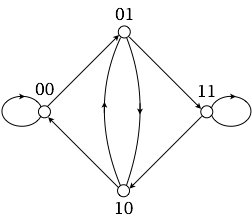
\includegraphics[scale=0.5]{FiguresGraph/dB2by2}
       \caption{The $4$-node, order-$2$ de Bruijn network.}
  \label{fig:dB2by2}
\end{center}
\end{figure}

\begin{figure}[hbt]
\begin{center}
       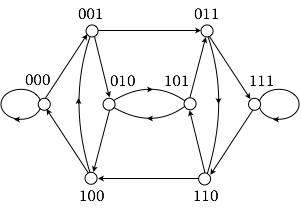
\includegraphics[scale=0.6]{FiguresGraph/dB2by3}
       \caption{The $8$-node, order-$3$ de Bruijn network.}
  \label{fig:dB2by3}
\end{center}
\end{figure}

For every integer $n \in \N^+$, the {\it order-$n$ de Bruijn network}
is the {\em directed} graph $\d_n$ whose nodes comprise the set of
length-$n$ binary strings.\footnote{While {\em binary} de Bruijn
  networks are the most frequently encountered ones, one can also find
  de Bruijn networks whose nodes comprise all length-$n$ strings over
  larger finite alphabets.  Such extended families also find
  applications in coding theory.}  The sets $\n_{\fd_2}$ and
$\n_{\fd_3}$ appear in (\ref{eqn:deBruijn-seq}).


$\d_n$ is a regular directed graph; its nodes all have in-degree $2$
and outdegree-$2$.  Each node of $\d_n$ is a binary string of
length $n \geq 1$; hence it can be written in the form $\beta x$,
where $\beta \in \{0, \ 1\}$ is a {\it bit} (short for {\it binary
  digit}) and $x$ is a length-$(n-1)$ binary string.

The $2^{n+1}$ arcs of $\d_n$ come in pairs specified as follows.  For
each $\beta \in \{0,1\}$ and for each length-$(n-1)$ binary string
$x$, $\d_n$ has the two arcs
\[ (\beta x \rightarrow x0) \ \ \ \mbox{ and } \ \ \ 
(\beta x \rightarrow x1)
\]
We enumerate $\a_{\fd_3}$ in (\ref{eqn:deBruijn-arcs}).
\begin{equation}
\label{eqn:deBruijn-arcs}
{\small
\begin{array}{|ccccc|}
\hline
\mbox{\sc Source node} & & \mbox{\sc Target node} & & \mbox{\sc Target node} \\
\hline \hline
{\displaystyle
\left.
\begin{array}{c}
000 \\
001 \\
010 \\
011 \\
100 \\
101 \\
110 \\
111
\end{array}
\right\}
} &
\mbox{\sc goes to} 
  &
{\displaystyle
\left\{
\begin{array}{c}
000 \\
010 \\
100 \\
110 \\
001 \\
011 \\
101 \\
111
\end{array}
\right.
}
  &
\mbox{\sc and to}
  &
{\displaystyle
\left\{
\begin{array}{c}
001 \\
011 \\
101 \\
111 \\
000 \\
010 \\
100 \\
110
\end{array} 
\right.
}
 \\
\hline
\end{array}
}
\end{equation}

For each $n \in \N^+$, $\d_n$ has diameter $n$.  To see why this is
true, note that following any one of $\d_n$'s arcs, say from node $x$
to node $y$, consists of ``rewriting'' the length-$n$ string $x$ as
the length-$n$ string $y$.  The diameter bound therefore follows by
showing that, for any two string-nodes of $\d_n$, say node $u$ and
node $v$, one can rewrite string $u$ as string $v$ by traversing a
sequence of arcs---i.e., a directed path---of length at most $n$.
Observe, for instance, that the path in $\d_3$ described schematically
as follows
\[ 000 \ \rightarrow \ 001 \ \rightarrow \ 011 \ \rightarrow \ 111 \]
leads node $000$ to node $111$, by rewriting string $000$ as string
$111$.  The diameter bound is now an immediate consequence of the
following result.  The result builds upon a notion that we have not
yet encountered but will study in some detail in
Section~\ref{sec:Hamiltonian-cycle}
\index{graph!Hamiltonian cycle} \index{Hamiltonian cycle}.

A {\it Hamiltonian cycle} in an $n$-node graph $\g$ is a length-$n$
cycle that contains every node of $\g$ precisely once.  A {\it
  directed Hamiltonian cycle} in an $n$-node digraph $\h$ is a
length-$n$ directed cycle that contains every node of $\h$ precisely
once.

\begin{prop}
\label{thm:deBruijn-Hamiltonian}
For all $n \in \N^+$, $\d_n$ contains a {\em directed Hamiltonian
  cycle}, 
\index{directed Hamiltonian cycle in a digraph}
i.e., a length-$2^n$ directed cycle of the form
\begin{equation}
\label{eq:deBruijn-cycle}
 x \ \rightarrow \ y_1 \ \rightarrow \ y_2 \ \rightarrow \cdots
\ \rightarrow \ y_{2^n-1} \ \rightarrow \ x
\end{equation}
that contains every node of $\d_n$ precisely once; i.e.:
\begin{itemize}
\item
$\{x, \ y_1, \ y_2, \ldots, \ y_{2^n-1}\} \ = \ \n_{\fd_n}$.
\item
All of the ``$y$-nodes'' that appear in cycle
(\ref{eq:deBruijn-cycle}) differ from $x$ and from each other.
\end{itemize}
\end{prop}

The simplest proof of this result has two steps, each of which
introduces a topic we have not yet developed.  We develop these concepts plus the proof in 
Section~\ref{Appendix:deBruijn-Hamiltonian}.

%{\Denis Add a word here about hamiltonian and Eulerian and refer to the appendix...}

\ignore{************

\noindent {\bf (1)}
%
For any directed graph $\g$, the {\it line digraph} \index{line graph}
\index{line digraph} of $\g$, denoted $\Lambda(\g)$, is the following
directed graph.
\begin{itemize}
\item
The nodes of $\Lambda(\g)$ are the arcs of $\g$:
\[ \n_{{\Lambda}({\cal G})} \ = \ \a_{\fg} \]
\item
For each pair of arcs of $\g$ of the form
\[ \big[a_{x,y} = (x \ \rightarrow \ y) \big] \ \ \ \mbox{ and } \ \ \ 
\big[a_{y,z} = (y \ \rightarrow \ z) \big]
\]
i.e, arcs such that the endpoint of the first arc is the source of the
second arc, $\Lambda(\g)$ contains an arc $(a_{x,y} \ \rightarrow
\ a_{y,z})$.
\end{itemize}
The relevance of this topic to this section is that the line graph of
every de Bruijn network $\d_n$ is the ``next bigger'' de Bruijn
network, $\d_{n+1}$.  Let us verify this claim.

\begin{prop}
\label{thm:deBruin-linegraph}
For all $n \in \N^+$,
$\d_{n+1}$ is the line digraph of $\d_n$: $\d_{n+1} \ = \ \Lambda(\d_n)$.
\end{prop}

\begin{proof}
Each node of $\Lambda(\d_n)$ is an arc of $\d_n$, hence has the form
\[ (\beta x \ \rightarrow \ x \gamma) \]
for $x$ a length-$(n-1)$ binary string and $\beta, \gamma \in
\{0,1\}$.  Let us associate node $\beta x \gamma$ of $\d_{n+1}$ with
this node of $\Lambda(\d_n)$.

\smallskip

Note first that each arc of $\d_{n+1}$ has the form
\[ (\delta y \varepsilon \ \rightarrow \ y \varepsilon \varphi), \]
where $y$ is a length-$(n-2)$ binary string and $\delta, \varepsilon,
\varphi \in \{0,1\}$.  By our association of nodes of $\d_{n+1}$ with
arcs of $\d_n$, this arc of $\d_{n+1}$ does, indeed, correspond to two
successive arcs of $\d_n$.   The first of these successive arcs
{\em enters} node $y \varepsilon$ of $\d_n$; the second {\em leaves}
that node.

Note next that, given any two successive arcs of $\d_n$, say
\[
(\rho \sigma z \ \rightarrow \ \sigma z \tau) \ \ \ \mbox { and } \ \ \
(\sigma z \tau \ \rightarrow \  z \tau \xi)
\]
where $z$ is a length-$(n-2)$ binary string and $\rho, \sigma, \tau,
\xi \in \{0,1\}$, there is, indeed, an arc of $\d_{n+1}$ of the form
\[ (\rho \sigma z \tau \ \rightarrow \ \sigma z \tau \xi) \]
This means that the digraph $\d_{n+1}$ is identical to the digraph
$\Lambda(\d_n)$, modulo a renaming of nodes and arcs.\footnote{Technically,
  we are asserting that the digraphs ${\cal D}_{n+1}$ and ${\Lambda}({\cal D}_n)$ 
  are {\it isomorphic} to one another.  The topic of
  graph isomorphism is beyond the scope of this text, but our informal
  description provides all the details one would need to formalize the
  described isomorphism.}

The described correspondence between the nodes and arcs of $\d_{n+1}$
and $\Lambda(\d_n)$ completes the proof.  \qed
\end{proof}

\begin{figure}[hbt]
\begin{center}
       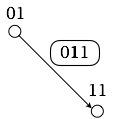
\includegraphics[scale=0.6]{FiguresGraph/dBlabelEdge}
\caption{Illustrating how to label each arc of a de Bruijn network by
  concatenating the labels of the nodes incident to the arc and
  compacting the common intermediate bits.  In the depicted example,
  the node-labels $01$ and $11$ combine to yield the arc-label $011$.}
  \label{fig:dBlabelEdge}
\end{center}
\end{figure}

\medskip

\noindent {\bf (2)}
{\it Eulerian cycles (or tours)}. \index{Eulerian cycle}
\index{Eulerian tour} A {\it directed Eulerian cycle} in a digraph
$\g$ is a directed cycle that contains each arc of $\g$ precisely
once.  We will see, later in this chapter, a truly elementary
argument, based on node-degrees, which proves that every de Bruijn
digraph has a directed Eulerian cycle.  This demonstration will
combine with Proposition~\ref{thm:deBruin-linegraph} to complete the
proof of Proposition~\ref{thm:deBruijn-Hamiltonian}.  \qed
%\end{proof}
********}

\bigskip

Stepping back from the structural specifics of $\d_n$, we now see that
de Bruijn networks provide us with a {\em
  bounded-degree---specifically, a degree-$2$} family of networks each
of whose constituent graphs has {\em logarithmic diameter}!  In this
regard, at least, de Bruijn networks have exactly the same
cost-performance as hypercubes---i.e., $2^n$-node graphs with diameter
$n$---with bounded degrees.  Even more dramatic, it has been shown
that sophisticated algorithmic techniques can achieve roughly
equivalent computational efficiency, on a broad range of significant
computational problems, using de Bruijn networks as using like-sized
hypercubes \cite{AnnexsteinBR90, BermondP89, Ullman84}.
